\documentclass[11pt,a4paper]{article}
\usepackage[a4paper,left=22mm,right=22mm,bottom=22mm,top=22mm]{geometry}
\usepackage{fontspec}
\usepackage[british]{babel}
\usepackage{amsmath,amssymb,graphicx,booktabs,array,tabularx,fancyhdr}
\usepackage[square,comma,numbers,sort&compress]{natbib}
\usepackage[hidelinks]{hyperref}
\usepackage{caption,subcaption}
\usepackage{float}
\usepackage{microtype}
\usepackage{xcolor}
\graphicspath{{figures/}}
\captionsetup{font=small,labelfont=bf}
\setlength{\parindent}{0em}
\setlength{\parskip}{0.4em}
\setlength{\headheight}{14pt}
\renewcommand{\topfraction}{0.9}
\renewcommand{\textfraction}{0.07}
\renewcommand{\floatpagefraction}{0.8}
\renewcommand{\bottomfraction}{0.8}
\setcounter{topnumber}{3}
\setcounter{bottomnumber}{3}
\setcounter{totalnumber}{5}
\pagestyle{fancy}
\fancyhead{}
\fancyhead[C]{\small Lab 9: Visual SLAM --- ORB-SLAM3, Kimera-VIO and LDSO}
\fancyfoot{}
\fancyfoot[C]{\thepage}
\renewcommand{\headrulewidth}{0pt}
\renewcommand{\abstractname}{Summary}
\newcommand{\studentname}{Team Fullcans}
% Monospace identifiers may break after underscores and dots.
\DeclareRobustCommand{\code}[1]{\begingroup\ttfamily\codebreaks#1\endgroup}
\newcommand{\codebreaks}{\renewcommand{\_}{\textunderscore\allowbreak}}
\setlength{\emergencystretch}{3em}
\title{Lab 9 Report\\[0.3em]\large Visual SLAM: information-matrix sparsity, ORB-SLAM, and a
comparison of ORB-SLAM3, Kimera-VIO and LDSO on EuRoC}
\author{\studentname}
\date{Revised: 23 November 2026}
\hypersetup{pdftitle={Lab 9 Report: Visual SLAM}}

\begin{document}
\maketitle
\noindent Repository: \url{https://github.com/monessss/2026Fall_TeamFullcans/tree/main/lab9}


\begin{abstract}
In the individual part we read the structure of a landmark-SLAM information matrix and
predict how marginalisation fills it in (D1), propose shortest-path initialisation for pose
graphs (D2), and summarise the ORB-SLAM architecture and its defences against wrong loop
closures (D3). We also answer the optional questions on LSD-SLAM (D4) and on reducing
landmark SLAM to a rotation-only problem (D5).
In the team part (D6), the archived stereo-inertial trajectories of ORB-SLAM3 and
Kimera-VIO are evaluated on EuRoC \code{MH\_01\_easy}. The ground-truth interval is
181.9\,s and 80.6\,m. Their exported world frames differ, so a rigid alignment is necessary.
After $\mathrm{SE}(3)$ alignment, body-position ATE RMSE is \textbf{3.9\,cm} for ORB-SLAM3
and \textbf{17.6\,cm} for Kimera-VIO. Aligning only the first associated pose gives
end-point errors of 1.8\,cm and 0.62\,m, respectively; the latter is about 0.8\,\% of
the associated reference path. These are observations from this sequence, not evidence
that either system is free of drift in general.
For optional D7, all trajectories and the reference are first expressed at the cam0
optical centre using the supplied body--camera extrinsic. After $\mathrm{Sim}(3)$ alignment,
ATE RMSE is 2.0\,cm for ORB-SLAM3, 17.1\,cm for Kimera-VIO, and 2.5\,cm for LDSO.
The archived LDSO output without loop correction has 3.8\,cm RMSE. The evaluation is
reproducible from committed trajectories; historical frame-processing and timing claims
are identified separately because the original runtime logs were not committed.
\end{abstract}

% Individual deliverables (D1--D5). Included from lab9_report.tex.
\section{Individual work}

\subsection{Deliverable 1: Spy game}\label{sec:d1}

We read the block pattern of the handout spy plot cell by cell (the pattern is stored in
\code{results/d1/spy\_pattern.txt}; Fig.~\ref{fig:spy}, left, redraws it). The matrix has
20 block rows: the thick lines separate 7 past poses, the current pose and the landmarks.
We call the poses $x_1,\dots,x_8$ and the landmarks $l_1,\dots,l_{12}$. The pose--pose
block is tridiagonal (odometry links $x_i$--$x_{i+1}$), the landmark--landmark block is
diagonal, and an off-diagonal pose--landmark block is non-zero iff the pose observed the
landmark. Table~\ref{tab:spy} lists the observations.

\begin{table}[H]
\centering\footnotesize\setlength{\tabcolsep}{3.5pt}
\begin{tabular}{lcccccccc}
\toprule
pose & $x_1$ & $x_2$ & $x_3$ & $x_4$ & $x_5$ & $x_6$ & $x_7$ & $x_8$ \\
\midrule
landmarks & $l_1,l_2$ & $l_1,l_2,l_4$ & $l_1,l_2,l_4$ & $l_1,l_3,l_4,l_6$ &
$l_3,l_4,l_5,l_6$ & $l_5,l_6,l_7,l_8$ & $l_6,l_8,l_9,l_{10}$ & $l_7,l_9,l_{10},l_{11},l_{12}$ \\
count & 2 & 3 & 3 & 4 & 4 & 4 & 4 & 5 \\
\bottomrule
\end{tabular}
\caption{Pose--landmark blocks of the D1 information matrix.}\label{tab:spy}
\end{table}

\begin{enumerate}
\item \textbf{8 robot poses} (7 past poses and the current one, $x_8$).
\item \textbf{12 landmarks.}
\item The current pose $x_8$ observes \textbf{5 landmarks}: $l_7, l_9, l_{10}, l_{11}, l_{12}$.
\item \textbf{The last pose $x_8$} observes the most landmarks (5); every other pose sees 2--4.
\item The 2nd landmark $l_2$ is observed by \textbf{$x_1$, $x_2$ and $x_3$}.
\item Marginalising a variable replaces the information matrix by the Schur complement, which
  connects all of the variable's neighbours with each other. The neighbours of $l_2$ are
  $x_1,x_2,x_3$. The links $x_1$--$x_2$ and $x_2$--$x_3$ already exist, so the only fill-in
  is a new \textbf{$x_1$--$x_3$ block} (and its transpose); row and column $l_2$ disappear and
  everything else stays the same (Fig.~\ref{fig:spy}, middle, fill-in in red).
\item The past poses $x_1,\dots,x_7$ form a connected chain, so eliminating all of them
  makes their whole Markov blanket a clique. The blanket is $x_8$ (odometry link from $x_7$)
  and every landmark that a past pose has seen, $l_1,\dots,l_{10}$. The result is a
  \textbf{fully dense $11\times11$ block over $\{x_8,l_1,\dots,l_{10}\}$}. Only $l_{11}$ and
  $l_{12}$, which only the current pose saw, keep their sparse rows (diagonal block plus the
  link to $x_8$) (Fig.~\ref{fig:spy}, right). This is why filtering approaches (EKF-SLAM,
  which keep only the current pose) end up with a dense covariance/information matrix.
\item A variable can be marginalised without fill-in iff its neighbours are already pairwise
  connected. In this matrix that holds for the landmarks seen by a single pose or by two
  consecutive poses: \textbf{$l_{11}$, $l_{12}$} (seen only by $x_8$), and also $l_3$ ($x_4,x_5$),
  $l_5$ ($x_5,x_6$), $l_8$ ($x_6,x_7$), $l_9$ and $l_{10}$ ($x_7,x_8$). Marginalising any pose
  creates fill-in, because a pose links its landmarks with each other and with the
  neighbouring poses, and those links do not exist yet (landmarks are never directly
  connected). We checked every case with a symbolic elimination in
  \code{scripts/make\_figures.py}.
\item Both images show the pose--pose block after eliminating all landmarks: poses $i$ and
  $j$ are linked iff they observed a common landmark.
  \begin{itemize}
  \item \textbf{Left (100 poses, density 0.40):} many poses share landmarks with
    other poses, including poses far apart in time (40\,\% block density). The robot kept seeing the
    same small set of landmarks for the whole run, so it was \emph{surveying a small
    area} (e.g.\ a single room, or moving back and forth/looping inside it). The reduced
    camera system has substantially more long-range coupling than the right-hand example;
    the actual factorisation cost depends on ordering and fill-in.
  \item \textbf{Right (about 850 poses, density 0.014):} the matrix is banded, so each
    pose only shares landmarks with poses close to it in time. The robot was
    \emph{exploring a large environment} (e.g.\ a long corridor or a large building) and
    rarely came back. The few off-diagonal segments are \emph{revisits/loop closures}: around
    poses 500--570 the robot revisited an area observed around poses 270--350 (the
    segment runs parallel to the diagonal, so it went through it in the same direction),
    and the short blocks near poses 0/630, 650/820 and 730/810 are brief revisits.
    The thicker blocks around poses 650--700 and 720--740 indicate longer shared visibility;
    slower motion or rotation are possible explanations, not unique conclusions.
  \end{itemize}
\end{enumerate}

\begin{figure}[H]
\centering
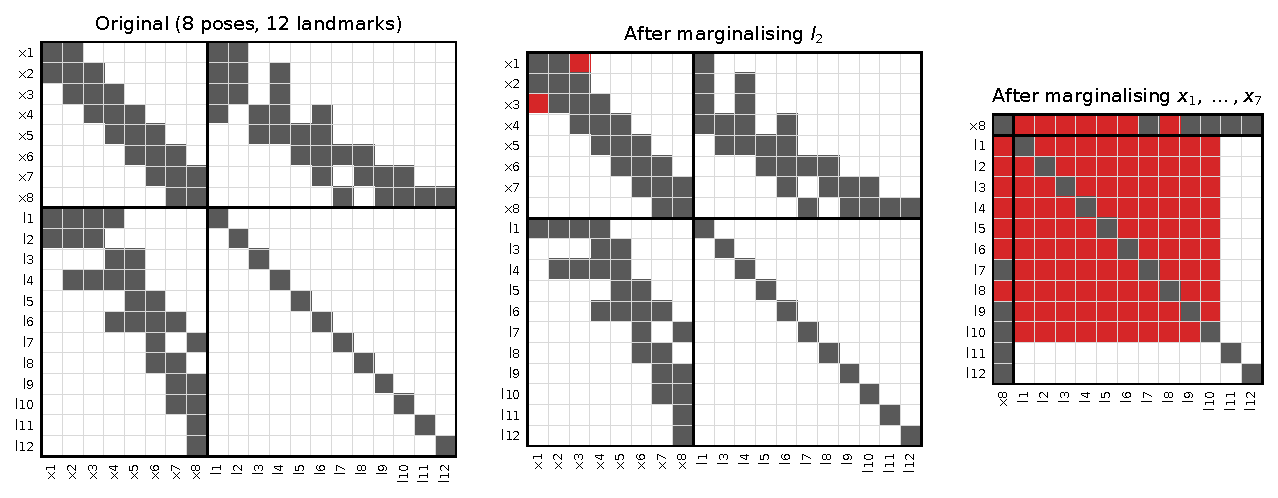
\includegraphics[width=\linewidth]{d1_spy_marginalization.pdf}
\caption{D1: block pattern of the handout matrix (left; poses $x$, landmarks $l$) and the
predicted pattern after marginalising $l_2$ (middle, question 6) and after marginalising
all past poses (right, question 7). Red blocks are fill-in created by the Schur complement.}
\label{fig:spy}
\end{figure}

\subsection{Deliverable 2: Well-begun is half done}\label{sec:d2}

\textbf{Proposal:} fix the root pose to the identity, compute a \emph{shortest-path
spanning tree} of the pose graph from the root (breadth-first search when all edges are
equally accurate; Dijkstra with edge weights equal to the measurement uncertainty, e.g.\
the trace of each edge's covariance, when they are not), and initialise every node by
composing the relative measurements along its tree path from the root.

\textbf{Rationale:} the initialisation error of a node grows with the number (and
uncertainty) of the measurements chained to reach it. Odometric chaining uses the path
$0\to1\to\dots\to i$, of length $i$. The shortest path also uses loop closures as
shortcuts, so on a graph with loops the hop count drops from $O(N)$ to the graph diameter,
and the accumulated noise drops with it. The method needs no special graph topology and
costs only $O(|\mathcal{E}|\log|\mathcal{V}|)$.

\subsection{Deliverable 3: Feature-based methods for SLAM (ORB-SLAM)}\label{sec:d3}

\paragraph{1. Modules (Fig.~1 of~\cite{murartal2015orb}).}
\begin{itemize}
\item \textbf{Map}: map points (3D position, viewing direction, representative ORB
  descriptor, scale-invariance range) and keyframes (pose, intrinsics, ORB features); the
  keyframes are connected by three graphs: the \emph{covisibility graph} (an edge when two
  keyframes share at least 15 map points), the \emph{spanning tree} and the sparse
  \emph{essential graph} (spanning tree, strong covisibility edges with at least 100
  shared points, and loop-closure edges).
\item \textbf{Place recognition}: a DBoW2 bag-of-words \emph{recognition database} of
  keyframes, built on an offline ORB \emph{visual vocabulary}; it is queried for
  relocalisation and for loop detection.
\item \textbf{Map initialisation}: computes a homography and a fundamental matrix in parallel
  from the first two frames, chooses one of them with a heuristic score, and builds the
  initial map by triangulation followed by full bundle adjustment.
\item \textbf{Tracking} (thread): extracts ORB features in every frame, estimates the
  camera pose from the previous frame with a constant-velocity model (or by global
  relocalisation when tracking is lost), refines it against the \emph{local map} (keyframes
  covisible with the current one) with motion-only BA, and decides whether to insert a new
  keyframe.
\item \textbf{Local mapping} (thread): processes new keyframes; it updates the covisibility
  graph, culls map points that are rarely found, triangulates new points from matches with
  covisible keyframes, runs \emph{local BA} on the current keyframe, its covisible keyframes
  and their points, and culls redundant keyframes (90\,\% of their points seen in at least
  three other keyframes).
\item \textbf{Loop closing} (thread): for each new keyframe, detects loop candidates with
  the bag-of-words database, computes the similarity transform $\mathrm{Sim}(3)$ to the loop
  keyframe (which also corrects scale drift), fuses the duplicated map points and
  corrects the poses on both sides of the loop, and finally optimises the \emph{essential
  graph} in $\mathrm{Sim}(3)$ to spread the loop correction over the whole map.
\end{itemize}

\paragraph{2. Wrong loop closures.}
ORB-SLAM accepts a loop only after several checks.
(i) \emph{Appearance}: a candidate keyframe must have a bag-of-words similarity higher than
the lowest similarity between the current keyframe and its covisible neighbours, and
keyframes already connected to the current one are excluded.
(ii) \emph{Temporal consistency}: a candidate is accepted only if three consecutive
keyframes produce loop candidates that are consistent, i.e.\ connected in the covisibility
graph.
(iii) \emph{Geometric verification}: ORB correspondences with the candidate are fed to
RANSAC with a $\mathrm{Sim}(3)$ solver (Horn's method); the transform is then refined, more
correspondences are searched with guided matching and the transform is optimised again. The
loop is accepted only with enough inliers (at least 40).

If a wrong loop passes these checks anyway, the method has no back-end mechanism to reject
it. The loop fusion merges map points that are actually different, and essential-graph
optimisation (a plain least-squares problem without robust kernels on the loop edges) pulls
the two places together. This bends and distorts the trajectory and the map
\emph{globally}. Later tracking and local BA are then done against a corrupted map, which
leads to more bad data associations and often to tracking failure. The error is not
undone later. This is why the checks above are very strict: ORB-SLAM gives up recall to
get near-perfect precision. Later systems added robust back-ends against outlier loops,
e.g.\ switchable constraints or pairwise consistency maximisation in Kimera-RPGO.

\subsection{Deliverable 4 (optional): Direct methods for SLAM (LSD-SLAM)}\label{sec:d4}

\paragraph{1. Modules of LSD-SLAM~\cite{engel2014lsd}.}
\begin{itemize}
\item \textbf{Tracking}: estimates the $\mathrm{SE}(3)$ pose of each new frame with respect to
  the current keyframe by minimising the variance-normalised photometric error over the
  pixels with depth (direct image alignment, Gauss--Newton on a pyramid).
\item \textbf{Depth map estimation}: refines the semi-dense inverse-depth map of the current
  keyframe with small-baseline stereo comparisons and filtering of tracked frames; when
  the camera moves too far, it creates a new keyframe by propagating the depth map to it.
\item \textbf{Map optimisation}: keyframes are added to a pose graph of $\mathrm{Sim}(3)$
  constraints, which come from direct $\mathrm{Sim}(3)$ image alignment between keyframes
  (with a depth residual, so scale drift is observable); the graph is optimised
  continuously in the background (g2o), and loop closures are found with FAB-MAP plus
  nearby keyframes.
\end{itemize}
\textbf{Similarities with ORB-SLAM:} keyframe-based design, separate tracking and mapping
threads, monocular input, $\mathrm{Sim}(3)$ pose graph to handle scale drift, appearance-based
loop detection with geometric verification. \textbf{Differences:} LSD-SLAM uses raw intensities
(photometric error) instead of ORB keypoints and reprojection error; it builds a
\emph{semi-dense} depth map (all pixels with enough gradient) instead of a sparse point map;
its back-end is a keyframe pose graph without bundle adjustment over the structure; and it
uses no descriptors, so its relocalisation is weaker.

\paragraph{2. Robustness.}
Feature-based methods are more robust to illumination changes and occlusions. Direct methods
assume brightness constancy: a change in exposure, auto-gain or lighting changes $I(p)$ and
biases the photometric error directly, unless one models affine brightness and calibrates
the camera photometrically as DSO does. Descriptors such as ORB/BRIEF use intensity
comparisons, which are invariant to monotonic brightness changes. Occluded points also simply fail to
match and are rejected by RANSAC or by robust kernels. In a direct method they become large
photometric residuals that enter a dense, non-convex alignment with a small convergence
basin. Direct methods can use image gradients outside repeatable keypoints and may therefore
help when keypoints are scarce; they still need informative gradients. Motion blur can
harm both methods, so it does not establish a general advantage for direct alignment.

\subsection{Deliverable 5 (optional): From landmark-based SLAM to rotation estimation}\label{sec:d5}

\paragraph{Elimination of translations and landmarks.}
Since the Euclidean norm is invariant to rotations, $\|R_i^\top v\|=\|v\|$, so the first two
terms of problem~(1) are equal to
\begin{equation}
\sum_{(i,k)\in\mathcal{E}_l}\|p_k-t_i-R_i\bar p_{ik}\|_2^2
+\sum_{(i,j)\in\mathcal{E}_o}\|t_j-t_i-R_i\bar t_{ij}\|_2^2 .
\end{equation}
Stack the positions $x=[t_1^\top\cdots t_N^\top\ p_1^\top\cdots p_M^\top]^\top\in\mathbb{R}^{3(N+M)}$
and consider the graph whose nodes are poses and landmarks and whose $E=|\mathcal{E}_l|+|\mathcal{E}_o|$
edges are the observation and odometry edges. Let $A\in\mathbb{R}^{E\times(N+M)}$ be its
incidence matrix (row $e=(a,b)$ has $-1$ in column $a$ and $+1$ in column $b$) and
$\bar A=A\otimes I_3$. Each measured vector enters as $R_i\bar m_e$ with $\bar m_e\in\{\bar p_{ik},\bar t_{ij}\}$,
and $R_i\bar m_e=(\bar m_e^\top\otimes I_3)\,\mathrm{vec}(R_i)$ is linear in the rotations.
With $r=[\mathrm{vec}(R_1)^\top\cdots\mathrm{vec}(R_N)^\top]^\top\in\mathbb{R}^{9N}$ there is a
constant sparse matrix $B\in\mathbb{R}^{3E\times 9N}$ (row block $e$ has
$\bar m_e^\top\otimes I_3$ in the column block of the observing pose $i$) such that the
stacked measurements are $Br$. Problem~(1) becomes
\begin{equation}
\min_{R_i\in\mathrm{SO}(3)}\ \min_{x}\ \|\bar A x - Br\|_2^2 + \sum_{(i,j)\in\mathcal{E}_o}\|R_j-R_i\bar R_{ij}\|_F^2 .
\end{equation}
For fixed rotations the inner problem is an unconstrained \emph{linear} least-squares
problem in $x$ (the rotation term does not depend on $x$). Fixing the gauge ($t_1=0$, i.e.\
removing the first column block of $\bar A$, which leaves $\bar A$ with full column rank if
the graph is connected), its minimiser is
$x^\star(r)=(\bar A^\top\bar A)^{-1}\bar A^\top B r$, and the minimum value is
$\|(I-\bar A(\bar A^\top\bar A)^{-1}\bar A^\top)Br\|^2=r^\top B^\top \Pi B r$, where
$\Pi=I-\bar A(\bar A^\top\bar A)^{-1}\bar A^\top$ is the orthogonal projector onto the
complement of the range of $\bar A$ (the cycle space of the graph). Substituting back, we get
the rotation-only problem
\begin{equation}
\min_{R_i\in\mathrm{SO}(3),\,i=1,\ldots,N}\ r^\top Q\, r+\sum_{(i,j)\in\mathcal{E}_o}\|R_j-R_i\bar R_{ij}\|_F^2,\qquad Q=B^\top\Pi B
\end{equation}
which depends on the rotations only. The original optimal translations and landmarks are
recovered in closed form as $x^\star(r^\star)$. The rotation term can also be written as a
quadratic form $r^\top (L_R\otimes I_3)\,r$ with a ``connection Laplacian'' of the odometry
graph, so the whole problem is $\min_{R\in\mathrm{SO}(3)^N} r^\top \tilde Q r$, a quadratic
problem over rotations.

\paragraph{Why the smaller problem is not necessarily faster.}
Local measurement factors make the original normal equations sparse. Eliminating all
positions can introduce long-range couplings between rotations, so an explicitly formed
$Q$ may be dense. A dense implementation can need $O(N^2)$ storage and $O(N^3)$ direct
factorisation, despite having fewer degrees of freedom. These are possible costs, not
universal bounds for SLAM: sparse factorisation depends on graph topology and elimination
ordering, and the projector can also be applied implicitly using sparse solves.
Fill-in is not inevitable for every graph (for a connected tree the translational
incidence matrix has no cycle-space residual). Thus the rotation-only formulation is not
guaranteed to be faster or slower; its structure and numerical implementation determine
whether the reduction is useful.


\section{Team work}\label{sec:team}

\subsection{Setup}\label{sec:setup}

We used the provided Docker images \code{orbslam:latest} (ORB-SLAM3~\cite{campos2021orbslam3},
\code{Stereo-Inertial/\allowbreak stereo\_inertial\_euroc} with the stock \code{EuRoC.yaml}, Pangolin viewer
enabled by the lab patch) and \code{kimera:latest} (Kimera-VIO~\cite{rosinol2020kimera} pinned at
commit \code{980ff72d}, since the \code{feature/prerelease} branch no longer exists; lab
\code{params/} unchanged, loop closure detection off, \code{--initial\_k=50 --final\_k=10000}).
The dataset is EuRoC~\cite{burri2016euroc} \code{MH\_01\_easy} (3682 stereo pairs at 20\,Hz, IMU at
200\,Hz). The containers are started with \code{run\_docker\_vnav.sh}, which maps our container
paths to the docker host and forwards the X display. The session notes describe successful GUI runs performed sequentially. The original
runtime logs and image digests were not committed, so those notes are not independent
verification of GUI behaviour or wall-clock performance. The revised launch scripts
record exit status and output hashes for future runs.

\textbf{One fix was needed for Kimera.} Kimera-VIO reads
\code{state\_groundtruth\_estimate0/\allowbreak sensor.yaml} with OpenCV's \code{FileStorage}, which only
accepts YAML files that start with \code{\%YAML:1.0}. The original EuRoC files do not have this
line, and the first run aborted with \emph{Cannot open file \dots/sensor.yaml}. We did not change
the SLAM code or the dataset. \code{scripts/run\_slam.sh} instead builds a hard-linked copy
\code{MH\_01\_easy\_kimera} (no extra disk space) in which only the \code{*.yaml} files get the
header, and runs Kimera on it with \code{run\_kimera.sh -p}.

The archived ORB-SLAM3 output contains 3678 poses spanning 183.85\,s; Kimera-VIO
contains 818 keyframe poses spanning 181.40\,s. This is consistent with broad sequence
coverage, but output timestamps alone cannot establish that every input frame was processed.
The session notes state that the full sequence was supplied; the Kimera launcher starts
at frame 50. The timestamp conversion divides ORB-SLAM3 nanoseconds by $10^9$ and converts
Kimera's CSV to TUM format. Both conversions were checked against the raw files.
Plots use \code{evo\_traj}~\cite{grupp2017evo}; error statistics use \code{evo\_ape --align}.
D6 compares body/IMU positions, with timestamp associations within 10\,ms: 3638 ORB-SLAM3
poses and 813 Kimera poses match the ground truth. Commands and metrics are provided in
\code{scripts/evaluate.sh} and \code{results/d6/metrics.json}.

\subsection{Deliverable 6: trajectories without alignment}\label{sec:d6a}

\begin{figure}[tbp]
\centering
\begin{subfigure}[b]{0.48\linewidth}
  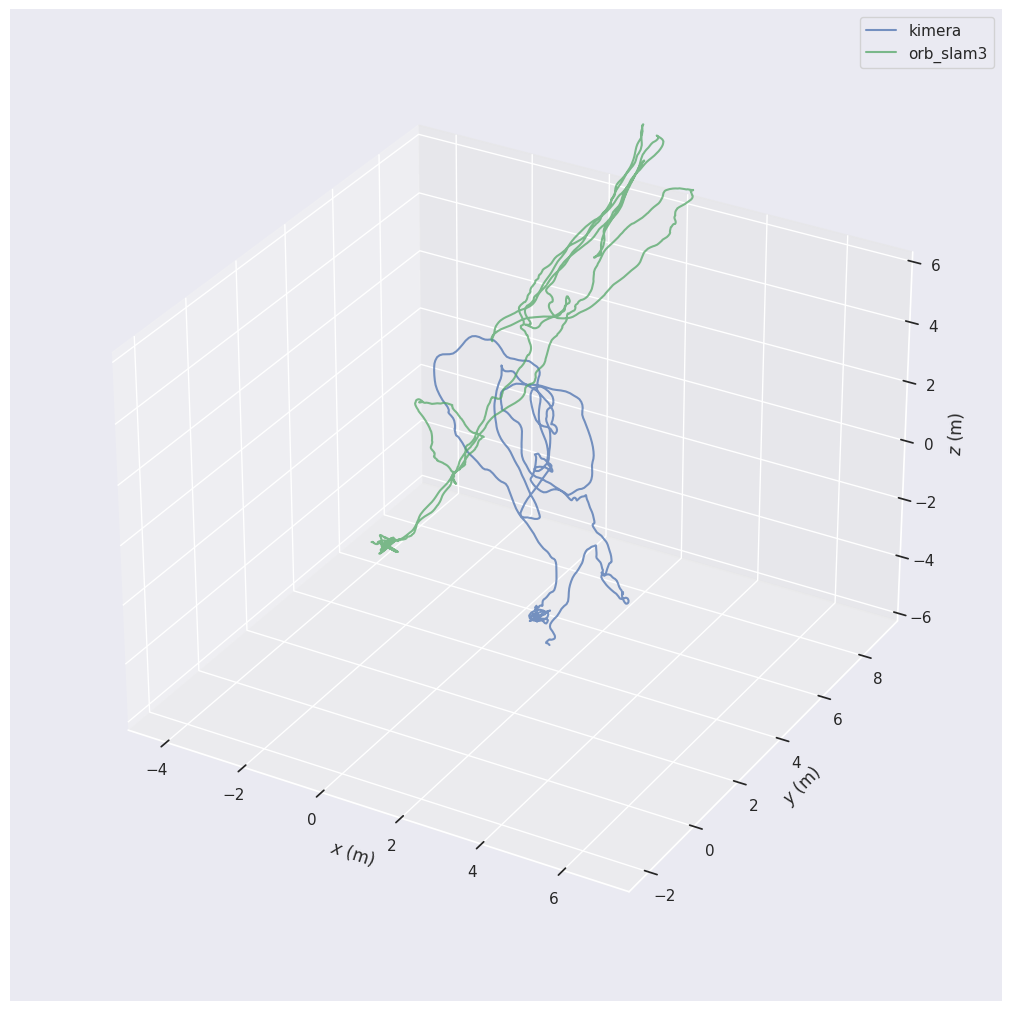
\includegraphics[width=\linewidth,trim=60 90 0 80,clip]{d6_evo_traj_unaligned.png}
  \caption{\code{evo\_traj tum kimera.txt orb\_slam3.txt --plot}}
\end{subfigure}

\vspace{0.4em}
\begin{subfigure}[b]{\linewidth}
  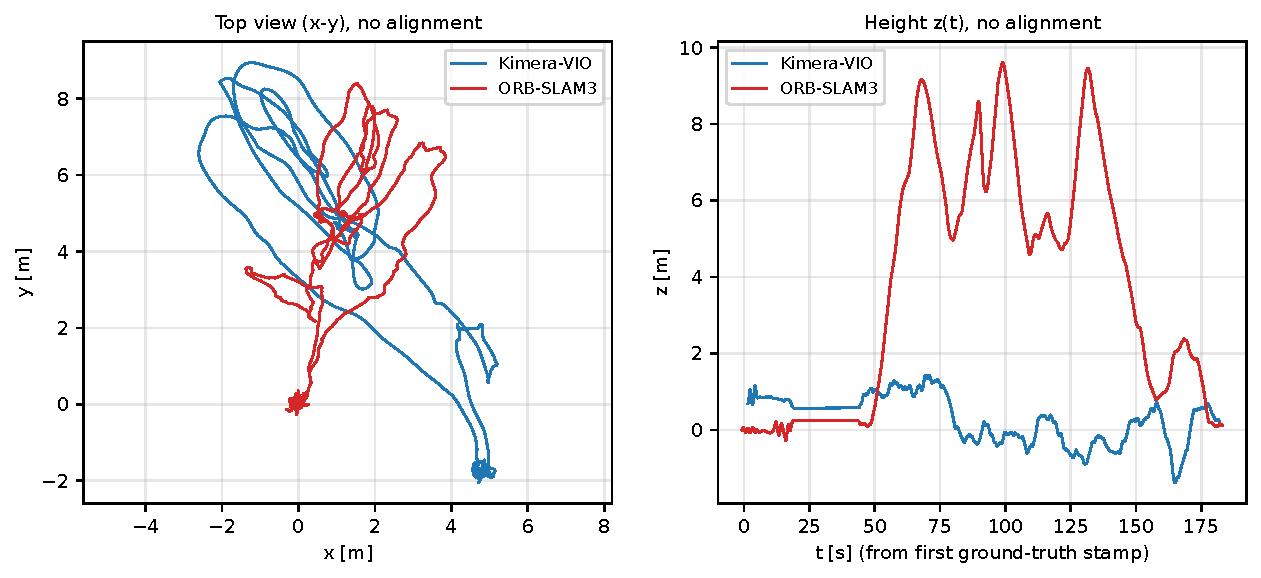
\includegraphics[width=\linewidth]{d6_unaligned.pdf}
  \caption{Same data: top view (dots mark the first pose) and height over time.}
\end{subfigure}
\caption{D6, no alignment: each trajectory is plotted in the world frame chosen by its own system.}
\label{fig:unaligned}
\end{figure}

\paragraph{What we see.} The two trajectories in Fig.~\ref{fig:unaligned} have similar lengths
(Kimera 79.1\,m, ORB-SLAM3 81.6\,m) and, after rotating one of them, the same shape, but they are
rotated, translated and tilted with respect to each other. Kimera starts at $(4.71,-1.79,0.69)$\,m
and moves in a nearly horizontal plane, with $z$ between $-1.3$ and $1.3$\,m. ORB-SLAM3 starts
exactly at the origin with identity orientation, and its ``height'' $z$ rises to 9.5\,m, which
the MAV did not fly: the motion that is horizontal in the real world appears along $z$ in the
ORB-SLAM3 frame. The two estimates are not wrong; they use \textbf{different world-frame
conventions}:
\begin{itemize}
\item \textbf{Kimera-VIO} initialises its state from the ground truth (\code{autoInitialize: 0}
  in \code{BackendParams.yaml}):
  its first pose is the ground-truth pose of frame 50. Its world frame therefore \emph{is} the
  EuRoC (Vicon/Leica) world frame, with $z$ against gravity. After that point it is pure
  odometry.
\item \textbf{ORB-SLAM3} (stereo-inertial) estimates gravity during IMU initialisation, but
  its \code{SaveTrajectory\allowbreak EuRoC} function writes every pose relative to the IMU pose of the \emph{first
  keyframe} ($T_{w b_0}^{-1} T_{w b_k}$). Its world frame is thus the body frame of the
  vehicle at start-up. In EuRoC the IMU $x$ axis points roughly up, so gravity is along
  $(-0.94,\,0.05,\,0.34)$ in this frame; the frame is tilted by $110^\circ$ with respect to
  the ground truth and its origin is the starting position.
\end{itemize}
The exported frames must be reconciled before comparison. In VIO, gravity constrains
roll and pitch while global yaw and position remain gauge freedoms. The large tilt here
comes from the body-relative export convention; it does not mean that gravity is
unobservable. We follow the handout's $\mathrm{SE}(3)$ alignment protocol.

\subsection{Deliverable 6: trajectories aligned with ground truth}\label{sec:d6b}

\begin{figure}[tbp]
\centering
\begin{subfigure}[b]{0.48\linewidth}
  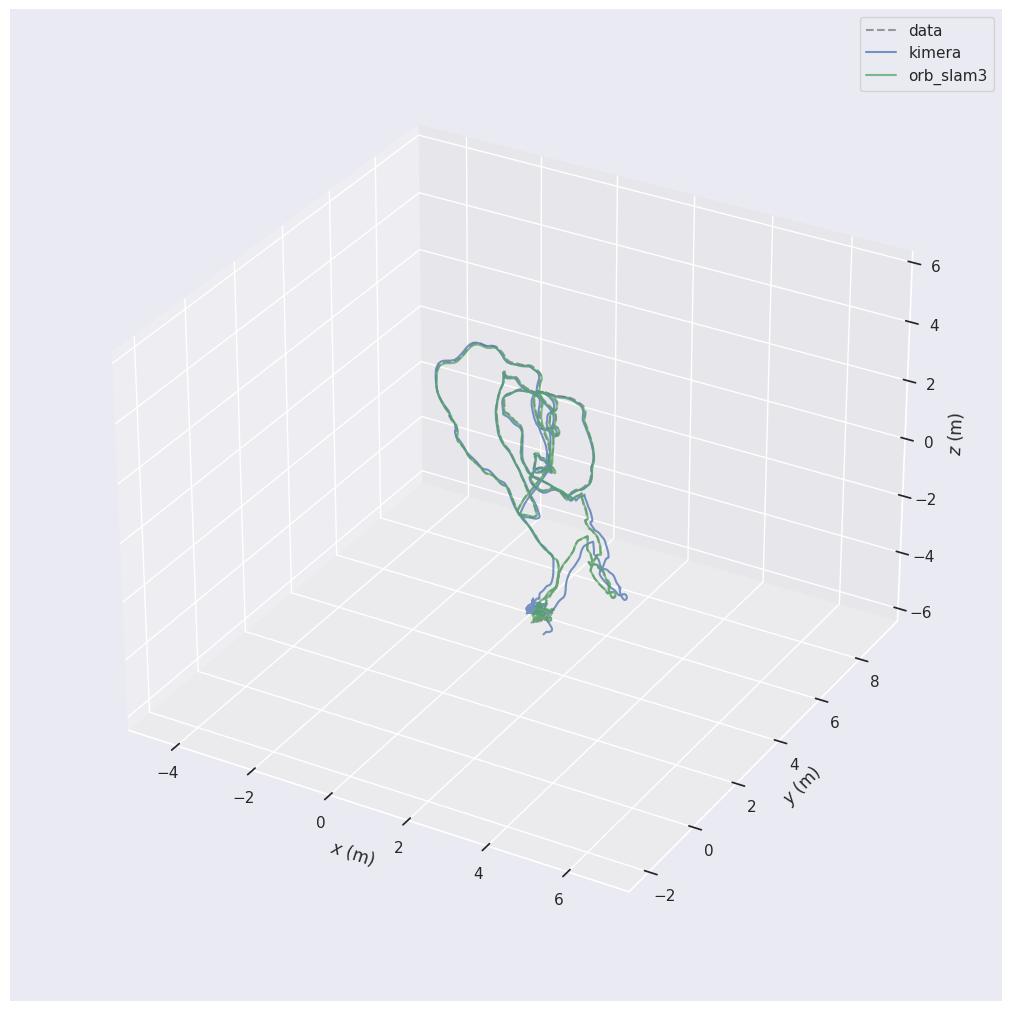
\includegraphics[width=\linewidth,trim=60 90 0 80,clip]{d6_evo_traj_aligned.png}
  \caption{\code{evo\_traj \dots --ref data.tum --plot --align}}
\end{subfigure}

\vspace{0.4em}
\begin{subfigure}[b]{\linewidth}
  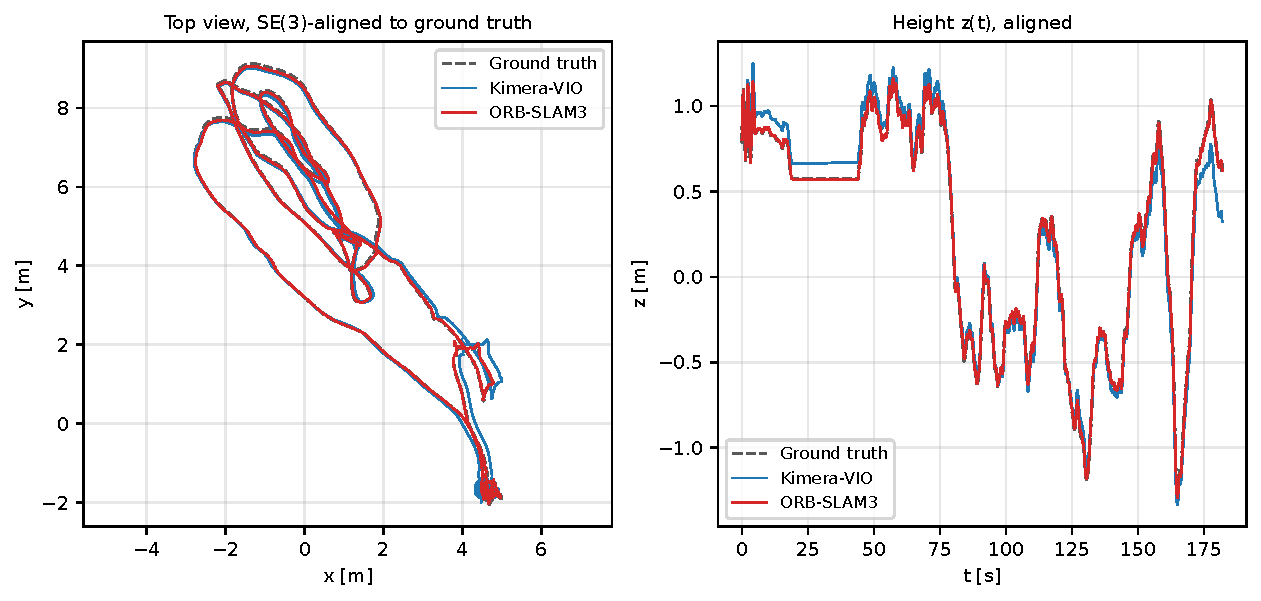
\includegraphics[width=\linewidth]{d6_aligned.pdf}
  \caption{Same data: top view and height, ground truth dashed.}
\end{subfigure}

\vspace{0.4em}
\begin{subfigure}[b]{\linewidth}
  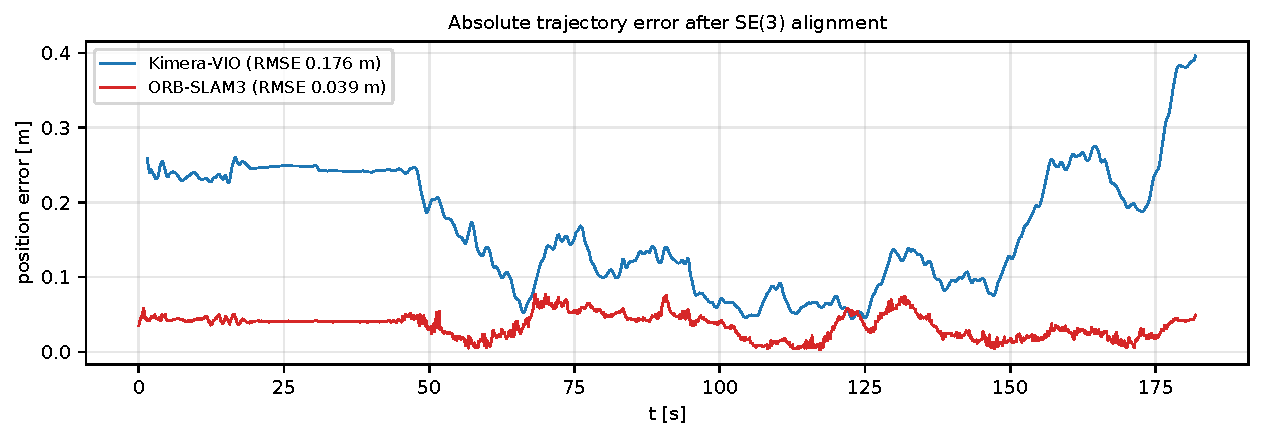
\includegraphics[width=\linewidth]{d6_ate_time.pdf}
  \caption{Position error over time after the $\mathrm{SE}(3)$ alignment (\code{evo\_ape --align}).}
\end{subfigure}
\caption{D6, after $\mathrm{SE}(3)$ alignment (Umeyama~\cite{umeyama1991}, no scale) of each estimate to the
EuRoC ground truth.}
\label{fig:aligned}
\end{figure}

\code{--align} solves for the rigid transformation $T\in\mathrm{SE}(3)$ that minimises
$\sum_k\|T p^{\text{est}}_k - p^{\text{gt}}_k\|^2$ over all associated positions. For Kimera this transformation is
almost the identity ($1.8^\circ$ of tilt, $0.3^\circ$ of yaw, 0.23\,m of translation), as expected
from its ground-truth initialisation. For ORB-SLAM3 it is the $110^\circ$ rotation plus the
$(4.67,-1.74,0.87)$\,m offset to the starting point. After alignment both trajectories lie on
top of the ground truth (Fig.~\ref{fig:aligned}), including the height profile, and the
differences are now visible only in the error plot and in Table~\ref{tab:ate}.

\begin{table}[H]
\centering\small
\begin{tabular}{lcc}
\toprule
 & Kimera-VIO & ORB-SLAM3 \\
\midrule
poses evaluated (rate) & 813 (keyframes, $\approx$4.5\,Hz) & 3638 (every frame, 20\,Hz)\\
ATE RMSE, $\mathrm{SE}(3)$ align [m] & 0.176 & \textbf{0.039} \\
ATE mean / median / max [m] & 0.157 / 0.136 / 0.396 & \textbf{0.035 / 0.040 / 0.077} \\
rotation error RMSE [deg] & 2.54 & \textbf{1.25} \\
ATE RMSE, $\mathrm{Sim}(3)$ align [m] & 0.170 & \textbf{0.021} \\
estimated scale factor $s$ & 1.011 & 1.008 \\
end-point error, first pose aligned [m] & 0.62 (0.78\,\% of path) & \textbf{0.018} \\
max.\ error, first pose aligned [m] & 0.62 (at the end) & 0.16 \\
\bottomrule
\end{tabular}
\caption{Accuracy on the full \code{MH\_01\_easy} sequence (\code{evo\_ape}, translation part unless
stated; \code{results/d6/evo/ape\_*.txt}, \code{results/d6/metrics.json}).}
\label{tab:ate}
\end{table}

\paragraph{Drift.} Kimera-VIO is run as visual-inertial odometry with loop closure disabled
(\code{USE\_LCD=0}), a fixed-lag backend, and IMU preintegration~\cite{forster2017preintegration}.
With the first associated pose aligned, its position error fluctuates but has an overall
increasing trend, reaching a maximum of 0.62\,m at the final matched sample. It is not
monotonic: the archived samples contain 360 decreases larger than $10^{-6}$\,m.
The full-trajectory $\mathrm{SE}(3)$ fit distributes error over the trajectory and gives a
smaller RMSE than the end-point error. ORB-SLAM3's first-pose-aligned error reaches
0.162\,m and ends at 0.018\,m; this is low accumulated error on this sequence, not zero drift.

\paragraph{Possible explanation.} ORB-SLAM3 can reuse mapped landmarks and optimise
local visual-inertial constraints, whereas this Kimera configuration has no global loop
correction. Map reuse is a plausible contributor to the observed difference, but the
experiment does not isolate it from frontend, backend and initialisation differences.
The session notes report no explicit ORB loop event, one map and 126 keyframes; without
the original log, these event counts are not independently verified. No causal attribution
or general ranking across environments is made from this single run.

\paragraph{Scale.} Stereo and sufficiently excited inertial measurements make metric
scale observable. This does not guarantee zero scale error or absence of scale drift.
The fitted global scale factors are 1.008 for ORB-SLAM3 and 1.011 for Kimera-VIO,
consistent with approximately metric trajectories. A single fitted scale does not measure
how scale error changes over time. Monocular LDSO needs scale correction because absolute
scale is unobservable from its image-only input.

\paragraph{Sampling and orientation.} Kimera outputs keyframes while ORB-SLAM3 outputs
frame poses, so the main statistics use different sample sets. As a sensitivity check,
linear interpolation at the same 813 Kimera timestamps gives SE(3) position RMSE of
0.03800\,m for ORB-SLAM3 and 0.17604\,m for Kimera. This supports the ordering on this
sequence but does not remove differences in system configuration. Rotation-error RMSE
after the position-based alignment is 1.25$^\circ$ and 2.54$^\circ$, respectively. The
experiment does not establish which orientation component causes most position error.
Timing numbers in the historical notes are not used as a performance benchmark; the
submitted Kimera flags enable point-cloud display and disable mesh display.

\subsection{Deliverable 7 (optional): LDSO}\label{sec:d7}

\paragraph{Setup.} LDSO~\cite{gao2018ldso} extends direct sparse monocular odometry
(DSO~\cite{engel2018dso}) with place recognition and a $\mathrm{Sim}(3)$ loop-correction graph.
The session notes identify upstream revision \code{9b0c48c}, bundled DBoW3/g2o, and
Pangolin v0.6. The build script now checks out that exact revision. Input is cam0 with
the supplied EuRoC calibration. The archived output contains 711 keyframes spanning
183.30\,s, with 696 matched to the reference; the cleaner drops no malformed rows.
The notes report a complete GUI run and 16 accepted loops, but the original runtime log
is unavailable. Those counts, processing completeness and runtime are not inferred from
keyframe timestamps. The two archived trajectories represent the exporter settings with
and without pose-graph correction. The implementation uses background threads, so it is
not described as a single-threaded system.

\paragraph{A common physical reference point.} LDSO exports camera poses, while the
stereo-inertial trajectories and EuRoC ground truth represent the body/IMU. For D7 we
therefore convert the body trajectories and the reference to cam0 before association:
\begin{equation}
T_{WC}=T_{WB}T_{BC},\qquad
p_{WC}=p_{WB}+R_{WB}t_{BC}.
\end{equation}
The supplied \code{LeftCameraParams.yaml} gives $\|t_{BC}\|=0.06890$\,m. This rotating
lever arm cannot generally be absorbed by a constant world-frame alignment. The conversion
is implemented in \code{scripts/trajectory\_frames.py}; original trajectories are retained.
All three systems are then aligned to the cam0 reference with $\mathrm{Sim}(3)$, using
\code{--align --correct\_scale --plot\_mode xy}. D6 remains a body-position comparison.

\begin{figure}[tbp]
\centering
\begin{subfigure}[b]{0.36\linewidth}
  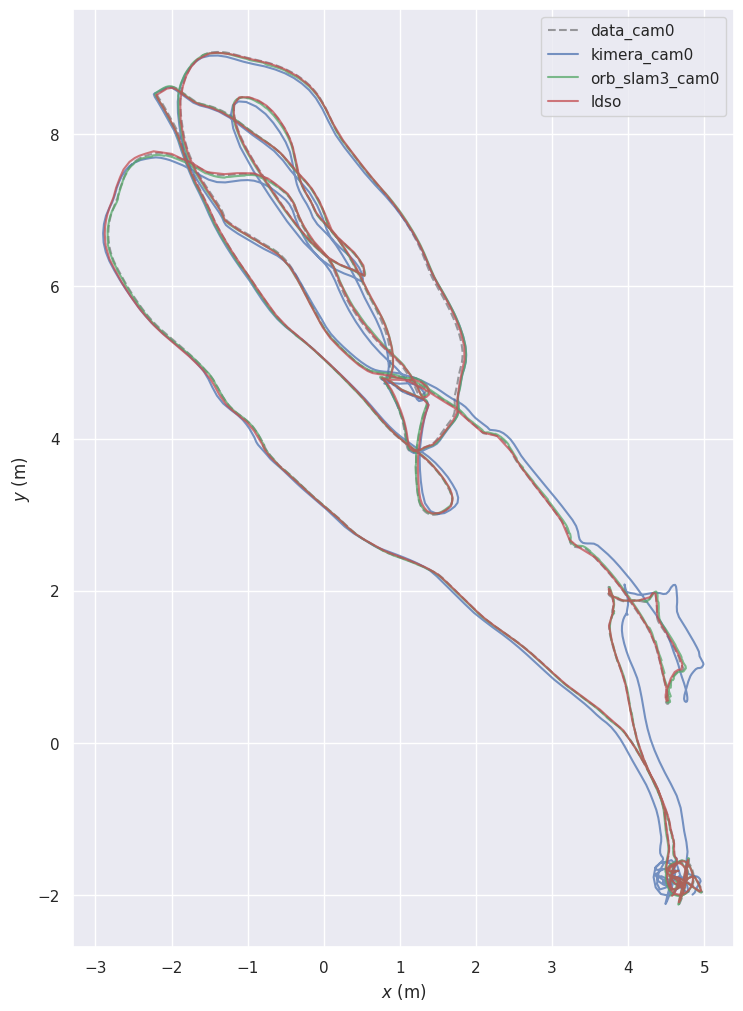
\includegraphics[width=\linewidth]{d7_evo_traj_sim3_xy.png}
  \caption{\code{evo\_traj} (\code{--align --correct\_scale --plot\_mode xy}).}
\end{subfigure}\hfill
\begin{subfigure}[b]{0.62\linewidth}
  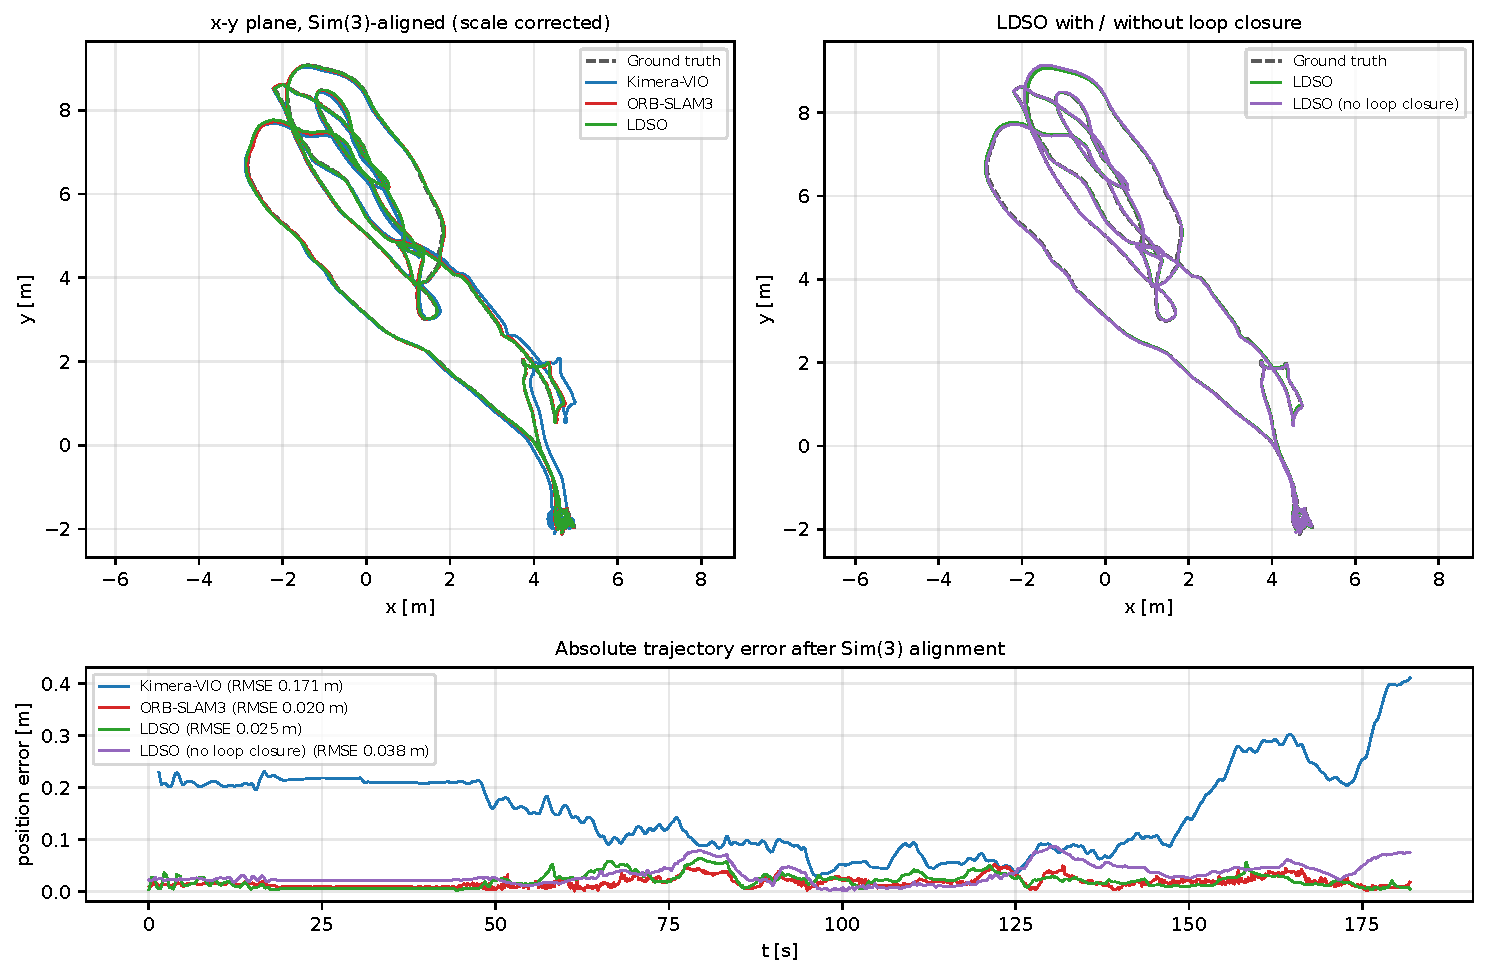
\includegraphics[width=\linewidth]{d7_sim3_aligned.pdf}
  \caption{Same alignment: x-y plane, LDSO with/without loop closure, and error over time.}
\end{subfigure}
\caption{D7: Kimera-VIO, ORB-SLAM3 and LDSO on \code{MH\_01\_easy}, each $\mathrm{Sim}(3)$-aligned
to the cam0 ground truth after sensor-frame conversion.}
\label{fig:d7}
\end{figure}

\begin{table}[tbp]
\centering\small
\begin{tabular}{lcccc}
\toprule
 & Kimera-VIO & ORB-SLAM3 & LDSO & LDSO, no loop \\
\midrule
sensors & stereo + IMU & stereo + IMU & mono & mono \\
poses evaluated & 813 & 3638 & 696 & 696 \\
raw cam0 path length [m] & 79.1 & 81.6 & 52.2 & 52.3 \\
$\mathrm{Sim}(3)$ scale factor $s$ & 1.011 & 1.008 & 1.530 & 1.540 \\
ATE RMSE, $\mathrm{Sim}(3)$ [m] & 0.171 & \textbf{0.020} & 0.025 & 0.038 \\
ATE max, $\mathrm{Sim}(3)$ [m] & 0.411 & \textbf{0.052} & 0.063 & 0.088 \\
ATE RMSE, $\mathrm{SE}(3)$ only [m] & 0.177 & 0.039 & 1.589 & 1.609 \\
\bottomrule
\end{tabular}
\caption{D7 cam0-position accuracy on associated archived samples (\code{results/d7/metrics.json},
\code{results/d7/evo/ape\_*\_sim3.txt}).}
\label{tab:d7}
\end{table}

\paragraph{Differences between the trajectories.}
\begin{itemize}
\item \textbf{Scale.} LDSO's raw path is 52.2\,m and the fitted scale is 1.530.
  Its camera-position RMSE is 1.589\,m with SE(3) only and 0.0253\,m with Sim(3).
  The large change shows the importance of scale correction; residual shape errors remain.
\item \textbf{Shape.} On their respective matched sample sets, cam0 Sim(3) RMSE is
  0.0204\,m for ORB-SLAM3, 0.0253\,m for LDSO and 0.1705\,m for Kimera. The first two
  trajectories overlap closely in the plot. All receive the same scale-fitting freedom
  in D7; D6 is the primary metric-scale comparison for the stereo-inertial systems.
  Different keyframe sampling and the use of one sequence limit generalisation.
\item \textbf{Loop-correction output.} The paired archived LDSO outputs have the same
  matched timestamps. Sim(3) RMSE changes from 0.0383 to 0.0253\,m, a reduction of
  about 1.30\,cm (34\,\%). Their fitted scales are 1.540 and 1.530. This supports a benefit
  from the exported loop-correction configuration on these samples; it does not verify
  an exact number or timing of accepted loop events.
\item \textbf{Effect of the reference-point correction.} Comparing LDSO directly to body
  truth gave 0.04295\,m RMSE (0.04872\,m without correction of the pose graph). Comparing
  it to camera truth gives 0.02531\,m and 0.03829\,m instead. The difference is an
  evaluation correction, not a new SLAM run or an algorithmic improvement.
\end{itemize}

\section{Conclusions}
Marginalisation can create fill-in between neighbours of eliminated variables, increasing
solver cost even when fewer variables remain. On the archived \code{MH\_01\_easy} data,
body-frame SE(3) alignment gives ORB-SLAM3 lower position RMSE than Kimera-VIO
(3.9\,cm versus 17.6\,cm). Map reuse is a plausible explanation, but was not isolated by
an ablation. Neither this comparison nor an end-point error establishes zero drift.
D7 requires both sensor-frame conversion and scale alignment. At the cam0 centre, LDSO
reaches 2.5\,cm Sim(3) RMSE versus 3.8\,cm for its archived no-loop output.
The corrected metrics and figures can be regenerated from the committed data. Full
processing counts, exact loop events and wall-clock performance need original or new
runtime logs; no such logs have been reconstructed from the old trajectories.

\section*{Individual responsibility}
Team: Team Fullcans. The individual deliverables D1--D5 are answered in
Section~1, and the team deliverables D6 and D7 (optional, LDSO) in Section~2.

\bibliographystyle{unsrtnat}
\bibliography{references}

\end{document}

